\documentclass{article}
\usepackage[utf8]{inputenc}
\usepackage[margin=1in]{geometry}
\usepackage{hyperref}
\usepackage{graphicx}
\usepackage{enumitem}
\usepackage{titlesec}
\usepackage{xcolor}
\usepackage{caption} % Handles caption centering
\usepackage{float}   % Provides the [H] specifier to lock image locations

% Color definitions
\definecolor{mdcblue}{RGB}{0, 50, 160}
\definecolor{darkgray}{RGB}{50, 50, 50}

% Hyperlink configuration
\hypersetup{
    colorlinks=true,
    linkcolor=mdcblue,
    urlcolor=mdcblue
}

% Title Formatting
\titleformat{\section}{\large\bfseries\color{mdcblue}}{\thesection}{1em}{}[\hrule height 0.5pt]
\titleformat{\subsection}{\normalfont\bfseries\color{darkgray}}{\thesubsection}{1em}{}

\begin{document}

% --- TITLE BLOCK ---
\begin{center}
    {\LARGE \bfseries Miami-Dade College Calorie Nutrition Tracker} \\[0.5em]
    {\large Project Documentation} \\[1.5em]
    \textbf{Prepared by:} Juan Carlos Ferrer Jr \\[0.5em]
    \textbf{Institution:} Miami-Dade College \\
    \textbf{Date:} \today
\end{center}

\vspace{1em}

% --- PROJECT DESCRIPTION ---
\section{Project Description}
The \textbf{Miami-Dade College Calorie Nutrition Tracker} is a desktop software application designed to help students track and manage their daily calorie intake. The application features an interactive dashboard displaying the user's daily target calorie limit, with flexibility to edit or adjust this limit as personal goals evolve. It provides a real-time visual comparison of \textit{Target Calories vs. Calories Consumed}, which dynamically updates whenever new items are logged or existing ones are removed.

% --- PROBLEM STATEMENT ---
\section{Problem Statement}
College students frequently face challenges in maintaining balanced nutrition due to demanding academic schedules, limited budgets, and a lack of straightforward, accessible health tools. Many existing commercial calorie trackers are bloated with unnecessary features, require paid subscriptions, or lack integration with campus life. Without an intuitive, free, and lightweight tool, students struggle to build consistent nutritional awareness, leading to poor dietary habits and lower energy levels required for academic success.

% --- FEATURES ---
\section{Features of the Application}
\begin{itemize}[leftmargin=*]
    \item \textbf{Dynamic Calorie Tracking Dashboard:} Real-time visual comparison between daily target calorie limits and current consumption.
    \item \textbf{Interactive Daily Food Log:} Displays all items consumed throughout the day, showing their respective calorie values alongside a \textbf{Delete/Remove} action button next to each entry for easy modifications.
    \item \textbf{Customizable Calorie Goal:} Direct interface options to edit and set a personalized daily calorie intake target.
    \item \textbf{My Foods Library:} A dedicated management page equipped with input fields for food names and numerical calorie amounts, allowing users to save custom items via an \textbf{Add Food} button.
\end{itemize}

% --- TECHNOLOGIES USED ---
\section{Technologies Used}
\begin{itemize}[leftmargin=*]
    \item \textbf{JavaFX \& JavaScript:} For UI presentation logic, dynamic layout binding, and event handling.
    \item \textbf{Figma:} Design prototyping and UI layout planning.
    \item \textbf{Google Gemini \& Google Stitch:} AI-assisted debugging, structural suggestions, and design refinement.
    \item \textbf{Microsoft Visual Studio Code:} Primary Integrated Development Environment (IDE) for code editing and project structure management.
    \item \textbf{Microsoft GitHub:} Version control system and remote repository hosting.
\end{itemize}

% --- SCREENSHOTS ---
\section{Screenshots of the Application}

\begin{figure}[H]
    \centering
    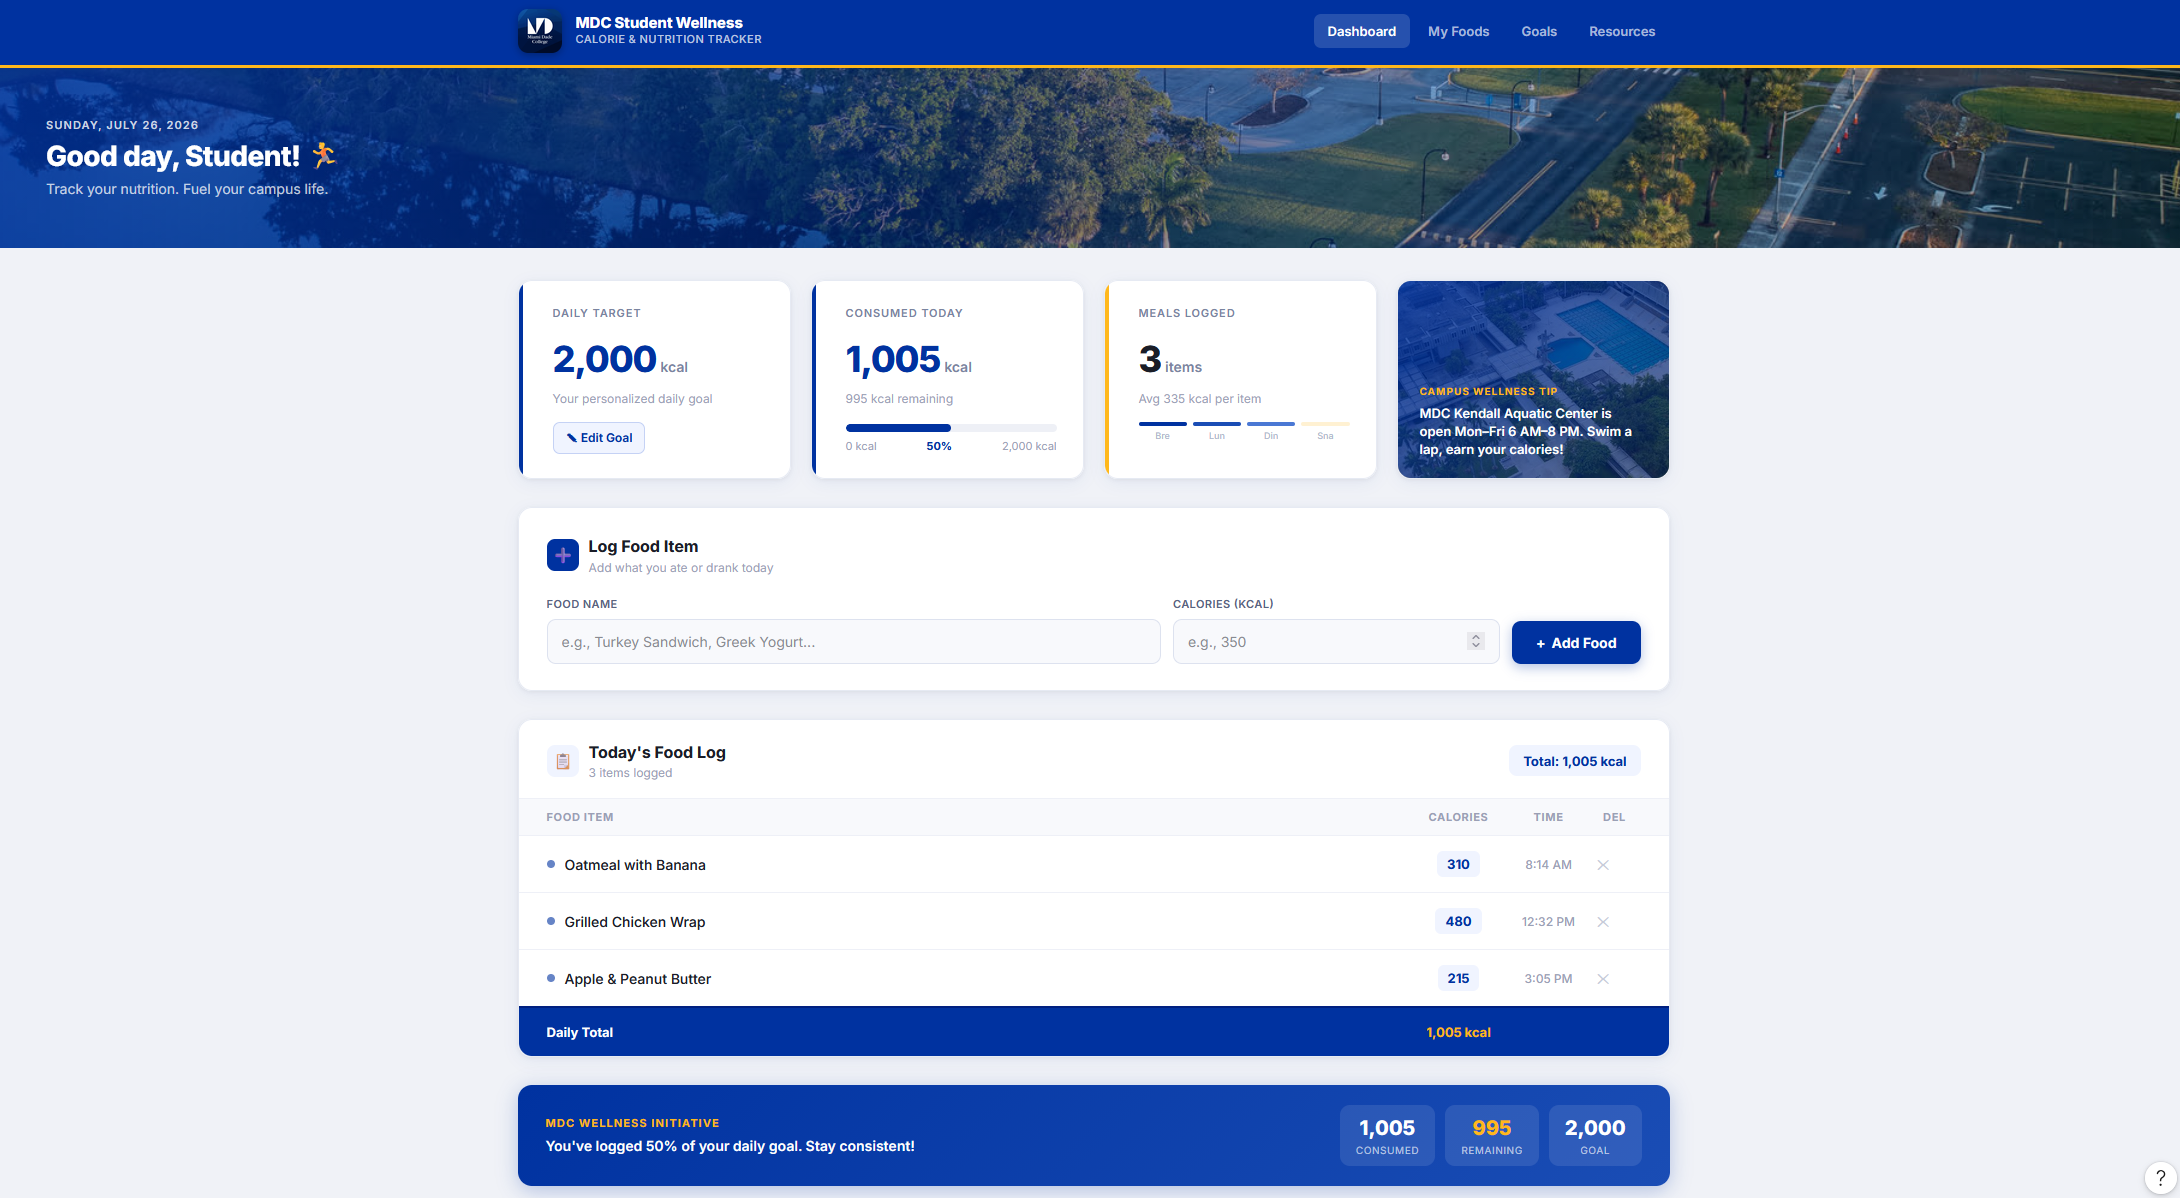
\includegraphics[width=0.75\linewidth]{screenshots/FigmaInspiration.png}
    \caption{Used through Figma Make to create a visualization of a home/landing page.}
    \label{fig:figma_home}
\end{figure}

\begin{figure}[H]
    \centering
    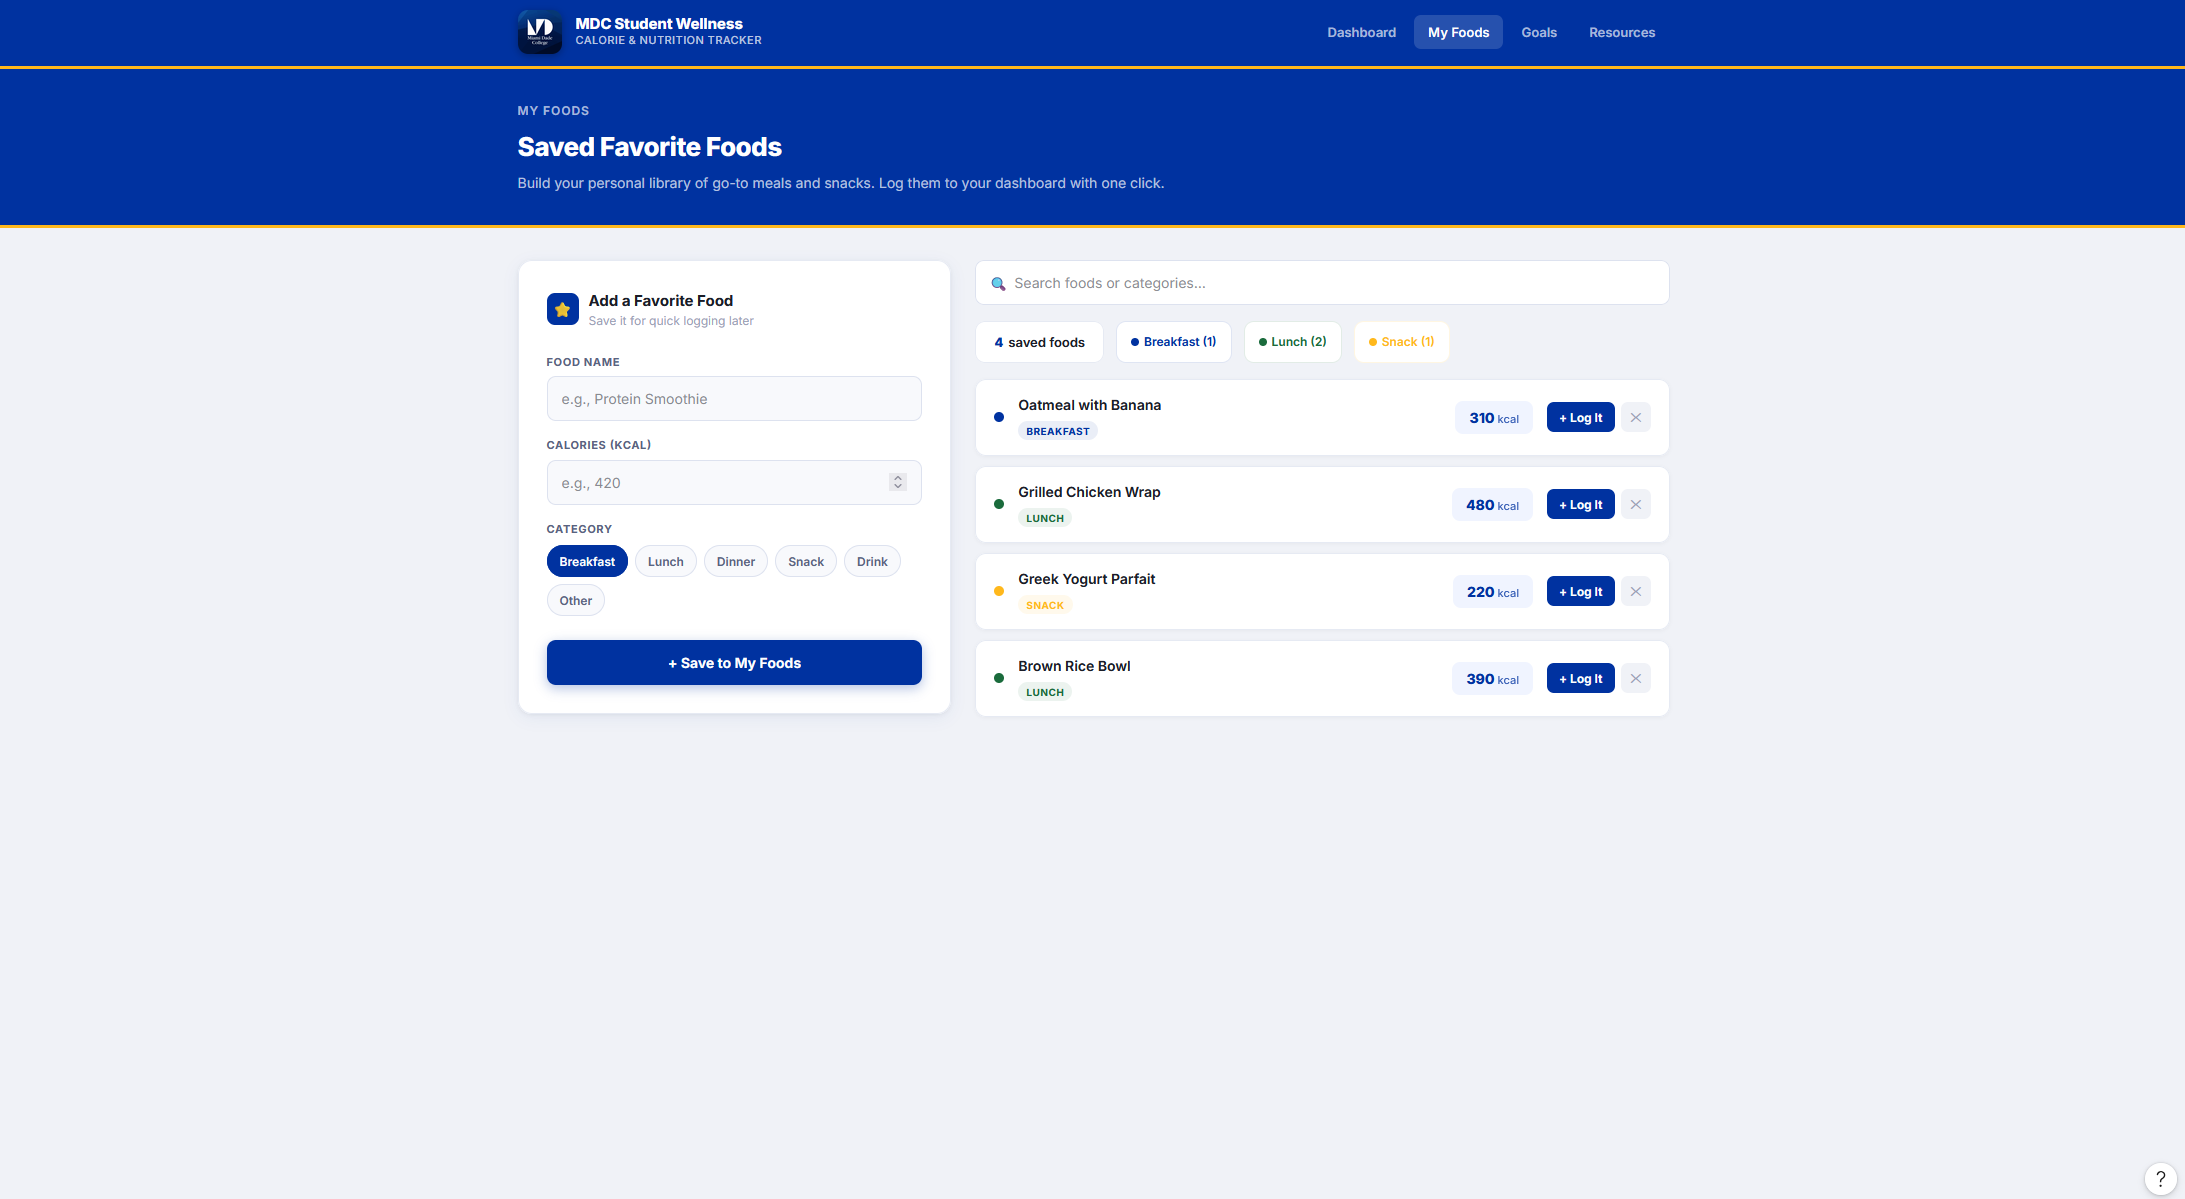
\includegraphics[width=0.75\linewidth]{screenshots/FigmaInspiration2.png}
    \caption{A secondary page with the objective to allow the user to add their own favorite foods.}
    \label{fig:figma_myfoods}
\end{figure}
    
\begin{figure}[H]
    \centering
    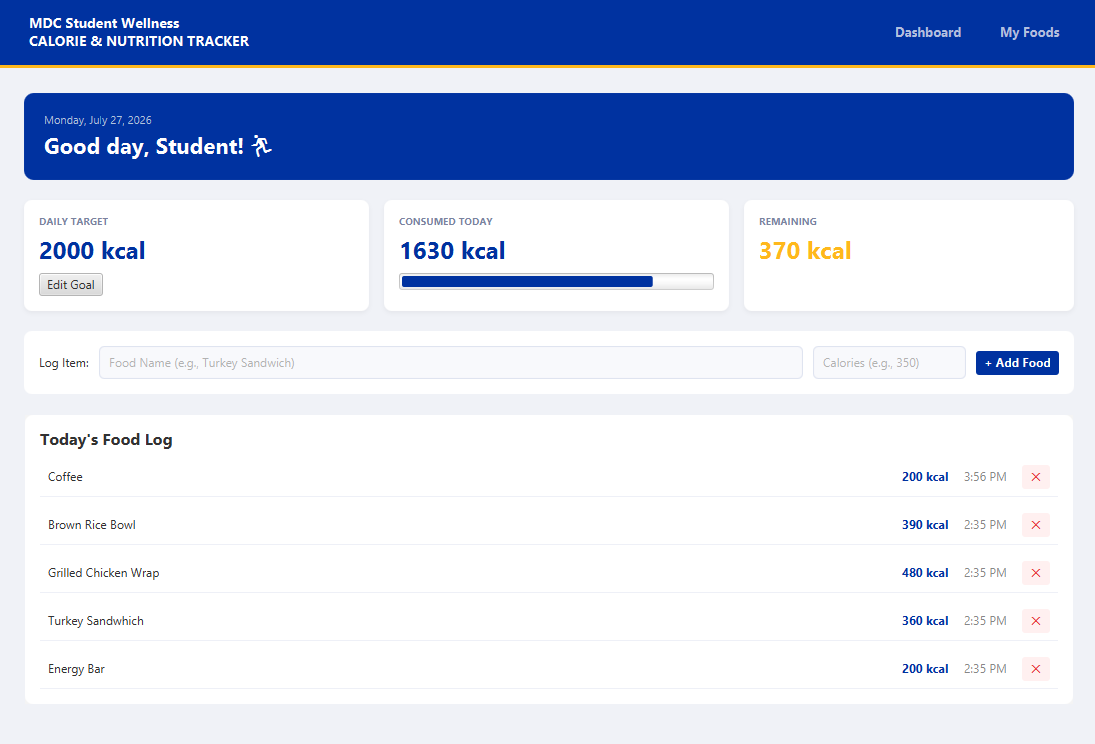
\includegraphics[width=0.75\linewidth]{screenshots/javafxhome.png}
    \caption{Java interpretation of the home/landing page.}
    \label{fig:javafx_home}
\end{figure}
 
\begin{figure}[H]
    \centering
    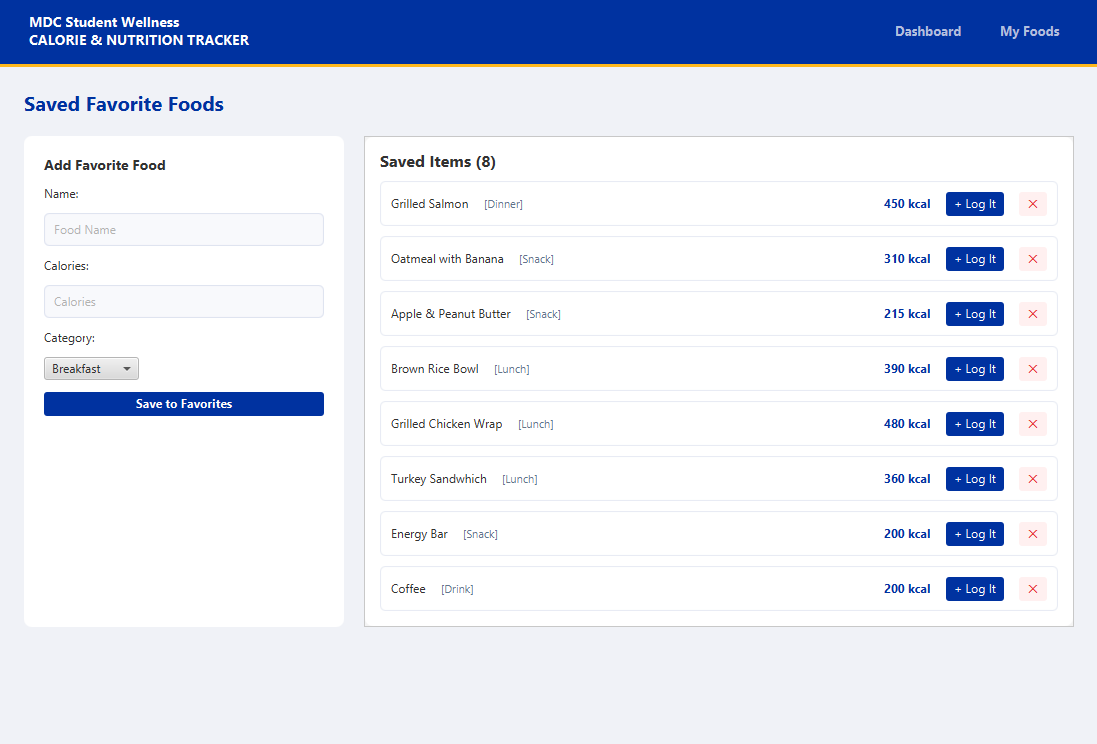
\includegraphics[width=0.75\linewidth]{screenshots/javafxmyfoods.png}
    \caption{Java interpretation of the My Foods page, allowing the user to add their own favorite foods to quickly add to the calorie tracker.}
    \label{fig:javafx_myfoods}
\end{figure}

% --- CHALLENGES AND SOLUTIONS ---
\section{Challenges Faced and Solutions}
As an introductory student to programming with JavaScript, handling syntax errors and compile-time issues proved to be the initial hurdle. Resolving these challenges required leveraging available technological tools—such as Google Gemini and IDE diagnostics—to troubleshoot errors, understand underlying programming concepts, and guide implementation choices. 

Throughout this process, a key takeaway was learning to balance the usage of automated assistance tools: using them not as a fundamental crutch, but rather as an essential, structured learning aid to build problem-solving autonomy.

% --- FUTURE IMPROVEMENTS ---
\section{Future Improvements}
\begin{itemize}[leftmargin=*]
    \item \textbf{Campus-Specific Enhancements:} Tailor visual elements and preset meal items specifically for tools provided to students enrolled at Miami-Dade College.
    \item \textbf{Calendar History Tracker:} Implement a historical log enabling users to review past daily calorie intakes over weeks or months.
    \item \textbf{Statistical Data Analysis:} Integrate charts and data analytics to provide actionable insights into macronutrient distribution and eating trends.
\end{itemize}

% --- COMPILATION INSTRUCTIONS ---
\section{Instructions on How to Compile and Run}
To run and test the application, access the experimental launcher using the following path in the official GitHub repository:

\begin{quote}
\verb|\mdccalorietracker\src\main\java\com\example\mdc\Launcher.java|
\end{quote}

\subsection*{Steps to Execute:}
\begin{enumerate}[leftmargin=*]
    \item Clone the repository from GitHub to your local machine.
    \item Open the project directory inside \textbf{Visual Studio Code} (or your preferred Java IDE).
    \item Ensure Java Runtime Environment (JRE) and JavaFX SDK are correctly configured in your environment path.
    \item Navigate to \texttt{Launcher.java} at the path above and run the file to launch the GUI application.
\end{enumerate}

\end{document}